\chapter{Quản Lý Dự Án}

\section{Quy trình phát triển phần mềm}
Nhóm thống nhất áp dụng quy trình phát triển phần mềm theo mô hình \textbf{Agile}, cụ thể là khung làm việc \textbf{Scrum}. Quy trình này giúp nhóm linh hoạt ứng phó với các thay đổi yêu cầu, tối ưu hóa hiệu suất làm việc của cả các thành viên và đảm bảo tiến độ chạy nước rút của dự án.

Hệ thống quản lý công việc được trực quan hóa thông qua bảng \textbf{Kanban (Jira)}. Toàn bộ các nhiệm vụ (Tasks) của dự án được phân rã khoa học từ cấp tính năng lớn xuống các đầu việc lập trình chi tiết, tương ứng với các mã định danh công việc từ \textbf{KAN-45 đến KAN-95} và được theo dõi nghiêm ngặt qua 3 trạng thái cốt lõi:
\begin{itemize}
    \item \textbf{To Do:} Danh sách các công việc chuẩn bị thực hiện trong Sprint.
    \item \textbf{In Progress:} Các công việc đang được các thành viên trong nhóm tập trung triển khai.
    \item \textbf{Done:} Các công việc đã hoàn thành, được Nhóm trưởng kiểm tra cấu trúc, rà soát mã nguồn (Code Review) và kiểm thử thành công trước khi đóng ticket.
\end{itemize}

\subsection{Phân biệt triết lý Agile và khung làm việc Scrum trong dự án}
Trong dự án AutoWashPro, nhóm áp dụng mối quan hệ tương hỗ giữa triết lý Agile và khung quản trị Scrum nhằm tối ưu hóa năng suất làm việc nhóm:
\begin{itemize}
    \item \textbf{Triết lý Agile (Agile Mindset):} Đóng vai trò là kim chỉ nam về tư duy, định hướng cho nhóm tinh thần sẵn sàng đón nhận sự thay đổi về yêu cầu chức năng từ phía Giảng viên hướng dẫn, ưu tiên việc bàn giao các phân hệ phần mềm chạy ổn định theo từng giai đoạn hơn là việc hoàn thiện các tập tài liệu quá dày mà thiếu tính thực tiễn.
    \item \textbf{Khung làm việc Scrum (Scrum Framework):} Đóng vai trò là công cụ triển khai cụ thể hóa tư duy Agile. Nhóm phân chia tổng thời gian phát triển thành các phân đoạn ngắn cố định (Sprints). Tại mỗi Sprint, nhóm thực hiện phân rã các yêu cầu thành hệ thống các thẻ công việc (Tickets) từ KAN-45 đến KAN-95 trên bảng Kanban trực quan để theo dõi sát sao chu trình phát triển sản phẩm.
\end{itemize}

% =================================================================
\section{Cấu trúc phân rã công việc (WBS Diagram)}
Để quản lý khối lượng công việc khổng lồ bao gồm cả phần lập trình phần mềm và phần phân tích mô hình nghiên cứu lý thuyết, nhóm tiến hành xây dựng Sơ đồ cấu trúc phân rã công việc (Work Breakdown Structure).

\begin{figure">[htbp]"
    \centering
    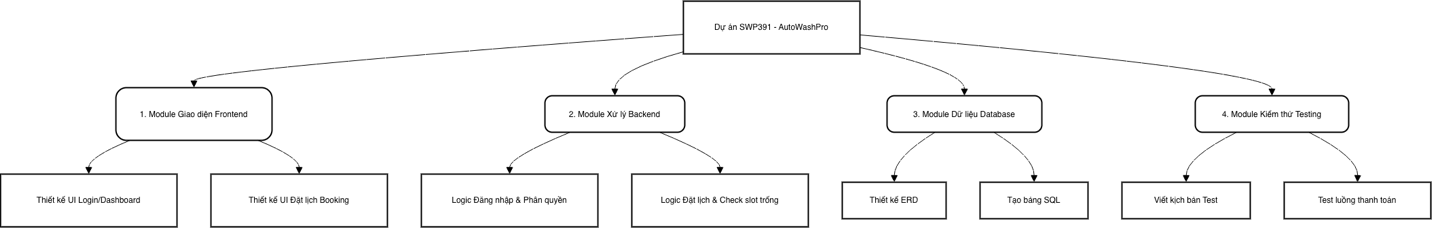
\includegraphics[width=0.95\textwidth]{images/wbs_diagram.png}
    \caption{Sơ đồ cấu trúc phân rã công việc WBS - Dự án AutoWashPro}
    \label{fig:wbs_diagram}
\end{figure}

Sơ đồ WBS trên được thiết kế theo cấu trúc cây phân cấp (Tree-structure), phân rã từ tên dự án tổng thể xuống các phân hệ module lớn (Xác thực, Đặt lịch, Tích điểm, Bảng điều khiển quản trị, Phân hệ thu thập log nghiên cứu), sau đó bẻ nhỏ thành từng task thực thi có thể định lượng được thời gian và công sức triển khai.

% =================================================================
\section{Kế hoạch tiến độ và Biểu đồ Gantt (Gantt Chart)}
Dựa trên cấu trúc phân rã WBS, nhóm thiết lập sơ đồ tiến độ thời gian thực hiện chi tiết cho từng hạng mục công việc xuyên suốt vòng đời của dự án. Tiến độ này giúp kiểm soát chặt chẽ các mốc thời gian (Milestones) quan trọng, đảm bảo không có đầu việc nào bị chậm trễ.

\begin{figure}[htbp]
    \centering
    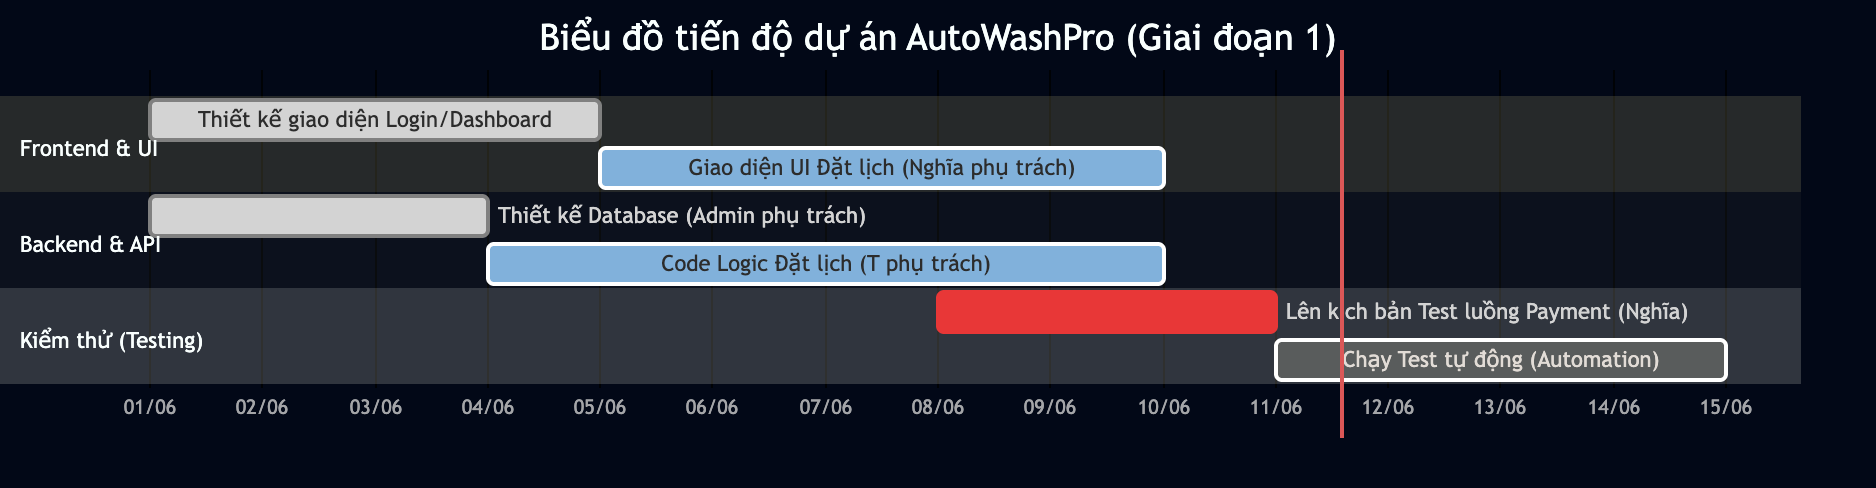
\includegraphics[width=1\textwidth]{images/gantt_chart.png}
    \caption{Biểu đồ Gantt tiến độ triển khai dự án chi tiết theo tuần}
    \label{fig:gantt_chart}
\end{figure}

Biểu đồ Gantt thể hiện rõ ràng dòng chảy thời gian, mối quan hệ phụ thuộc giữa các tác vụ (công việc nào làm trước làm nền tảng, công việc nào làm sau) và phân định rõ ràng nhân sự chịu trách nhiệm chính nhằm tối ưu hóa tính minh bạch trong quản trị dự án.

% =================================================================
\section{Cơ cấu nhân sự và Vai trò trong nhóm}
Để dự án vận hành mượt mà, các thành viên trong nhóm được phân bổ vai trò rõ ràng dựa trên năng lực chuyên môn và mục tiêu đóng góp:

\begin{enumerate}
    \item \textbf{Lê Nguyên Kiên (Nhóm trưởng / Project Manager / Backend Core):} Chịu trách nhiệm điều phối chung, thiết lập cấu trúc tài liệu LaTeX báo cáo, quản lý tiến độ mã nguồn trên GitHub, quản trị bảng việc Jira và thiết kế cấu trúc nền tảng Server API.
    \item \textbf{Lê Thị Quỳnh Nhung (NQ - Business Analyst / Documentation):} Phụ trách khảo sát, phân tích chi tiết yêu cầu hệ thống (SRS), đặc tả quy trình nghiệp vụ và xây dựng các sơ đồ Use Case, Activity.
    \item \textbf{Phan Triều Cường (LK - Database Engineer):} Phụ trách khảo sát cấu trúc thực thể, thiết kế chi tiết cơ sở dữ liệu quan hệ MySQL, chuẩn hóa cấu trúc các bảng thuộc tính và tối ưu hóa index truy vấn dữ liệu.
    \item \textbf{Trần Tiến Dũng (DT - Backend Developer):} Chịu trách nhiệm hiện thực hóa các sơ đồ tuần tự (Sequence Diagram), lập trình phát triển hệ thống các API endpoints cốt lõi và tích hợp logic tính toán hóa đơn nội bộ.
    \item \textbf{Lê Sỹ Nghĩa (T - Frontend Developer):} Phụ trách xây dựng giao diện ứng dụng phía Client (Web Responsive) cho các phân hệ đăng ký, quản lý phương tiện và đặt lịch dịch vụ trực tuyến.
    \item \textbf{Thành viên 6 (Frontend UI Developer):} Phụ trách chuyển đổi các bản thiết kế wireframe từ Figma thành giao diện trang quản trị Admin Dashboard trực quan cho nhân viên quầy.
    \item \textbf{Thành viên 7 (Quality Assurance / Tester):} Xây dựng tài liệu kịch bản kiểm thử (Test Cases), thực hiện kiểm thử đơn vị (Unit Test), kiểm thử tích hợp (Integration Test) và quản lý tiến độ sửa lỗi.
\end{enumerate}

% =================================================================
\section{Bảng phân công nhiệm vụ chi tiết (Jira Mapping)}
Dưới đây là bảng tổng hợp phân công công việc cụ thể cho các thành viên dựa trên hệ thống dải mã thẻ công việc đã được đồng bộ hóa và cấu hình chặt chẽ trên bảng quản trị Jira board:

\begin{table}[htbp]
\centering
\caption{Bảng phân công nhiệm vụ thành viên theo mã định danh KAN}
\label{tab:jira_mapping}
\begin{spacing}{1.2}
\small
\begin{tabular}{cllp{4.5cm}c}
\toprule
\textbf{STT} & \textbf{Thành viên} & \textbf{Mã vai trò} & \textbf{Nhiệm vụ phụ trách chính} & \textbf{Dải Ticket Jira} \\
\midrule
1 & Lê Nguyên Kiên & Lead / PM & Quản trị dự án, Setup LaTeX, Core API Backend & KAN-45 $\rightarrow$ KAN-52 \\
2 & Lê Thị Quỳnh Nhung & NQ - BA & Đặc tả yêu cầu SRS, Thiết kế sơ đồ Use Case, Activity & KAN-53 $\rightarrow$ KAN-61 \\
3 & Phan Triều Cường & LK - DB & Thiết kế Sơ đồ ERD, Chuẩn hóa Database Schema & KAN-62 $\rightarrow$ KAN-70 \\
4 & Trần Tiến Dũng & DT - BE & Thiết kế Sơ đồ Tuần tự, Lập trình API chức năng & KAN-71 $\rightarrow$ KAN-79 \\
5 & Lê Sỹ Nghĩa & T - FE & Phát triển giao diện UI/UX Client và Form đặt lịch & KAN-80 $\rightarrow$ KAN-87 \\
6 & Thành viên 6 & FE Admin & Phát triển giao diện Admin Dashboard quản trị & KAN-88 $\rightarrow$ KAN-91 \\
7 & Thành viên 7 & QA / Tester & Thiết kế kịch bản kiểm thử, chạy Unit/UI Test & KAN-92 $\rightarrow$ KAN-95 \\
\bottomrule
\end{tabular}
\end{spacing}
\end{table}